\documentclass[dvipsnames]{beamer}
\usepackage[T1]{fontenc}
\usepackage[utf8]{inputenc}
\usepackage[english]{babel}
\usepackage{graphicx}

\title{\large Deep Unsupervised Representation Learning on Protein
Sequences using Variational Autoencoders}
\author{{Emil Petersen} \and {Victor Nordam Suadicani}}
\usepackage{niceslides}

\begin{document}

\frame{\titlepage}

\begin{frame}{Overview}

\begin{block}{Idea}
Exploit deep learning to develop unsupervised representations of protein sequences.

This is desirable because it (potentially) yields a scalable, data-efficient process to capture useful protein features that can be used for downstream tasks in protein analysis. Some representations allow for exploration in protein space along properties of interest.
\end{block}

\begin{block}{Objectives}
\begin{itemize}
    \item Understand theory. Survey current approaches and relate to theory. Identify strengths and weaknesses.
    \item Apply to protein sequence domain and evaluate performance.
    \item Ideally, produce improved models. See approaches.
\end{itemize}
\end{block}
\end{frame}

\begin{frame}{Approaches}
    \begin{block}{Trade-offs}
    \begin{itemize}
        \item Aligned vs. variable length input sequences.
        \item Local vs. global representations: learning truly general properties of entire natural protein space, or focus on protein family.
        \item Can we translate representations back to proteins? Depends on the design.
    \end{itemize}
    \end{block}
    
    \begin{block}{Approaches (so far)}
    \begin{itemize}
        \item VAE: Aligned, local, latent space based representations.
        \item UniRep: Unaligned, global, mean-based (proteins not recoverable from representations).
        \item WaveNet: Unaligned, local, auto-regressive (convolutions). Direct sequence-to-sequence model, but an inner representation could potentially be extracted.
    \end{itemize}
    \end{block}
\end{frame}

\begin{frame}{Preliminary results}
    \begin{itemize}
        \item Our VAE with Bayesian decoder parameters achieves $\approx 0.72$ $\rho$ correlation on mutation effect prediction ($\beta$ lactamase family). Comparable to existing results, but room for improvement.
        \item UniRep pretrained globally, fine-tuned locally performs significantly worse. Around 0.37 $\rho$. Result is not final; there are significant details in finetuning left.
        \item WaveNet is originally used for sound, but has shown promising results (by others) on proteins ($\geq 0.7 \rho$). Currently working on this.
    \end{itemize}
\end{frame}

\begin{frame}{Projection of VAE representations}
\begin{figure}
    \centering
    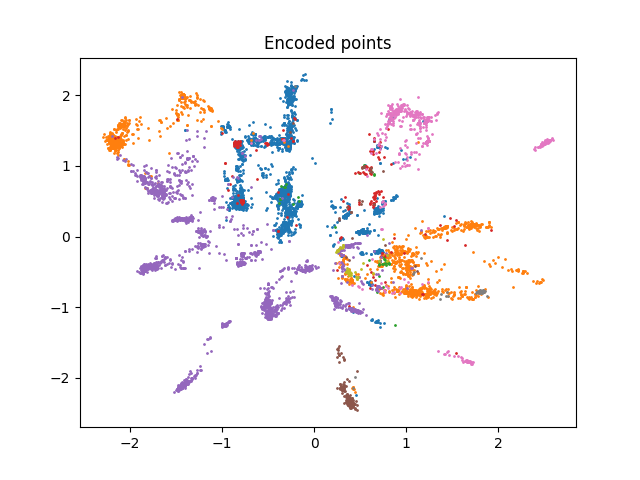
\includegraphics[width=0.9\linewidth]{presentation/vae.png}
\end{figure}
    
\end{frame}

\end{document}
